\documentclass[a4paper, 11pt]{article}
\usepackage{comment} % enables the use of multi-line comments (\ifx \fi) 
\usepackage{lipsum} %This package just generates Lorem Ipsum filler text. 
\usepackage{fullpage} % changes the margin
\usepackage{booktabs}
\usepackage{graphicx}
\usepackage{float}
\usepackage[brazilian]{babel}
\usepackage[utf8]{inputenc}
\usepackage[T1]{fontenc}

\begin{document}
%Header-Make sure you update this information!!!!
\noindent
\large\textbf{INF01145 - Fundamentos de Bancos de Dados} \hfill \\
\normalsize Relatorio 1 \hfill Ana C. Pagnoncelli, Rafael B. Audibert \\
Profª. Karin Becker \hfill 02/07/2019 \\

%% ===================================
\section*{Enunciado do trabalho}

O trabalho prático da disciplina deve versar sobre o projeto e uso de uma base de dados para um sistema de informação (SI), a
ser modelado e implantado em computador. O trabalho envolve a modelagem e o projeto da base de dados com o uso de
ferramentas de modelagem, bem como criação, instanciação e manipulação em um modelo relacional.

Esse relatório se refere à primeira parte do trabalho, dizendo respeito à implementação de um projeto conceitual da Base de Dados e sua subsequente implementação em SGBD relacional.

%% ===================================
\section*{Universo de Discurso}
O universo de discurso é baseado no site/aplicativo Google Play\cite{GooglePlay}, que é um serviço de distribuição digital de aplicativos, jogos, filmes, programas de televisão, músicas e livros, desenvolvido e operado pela Google\cite{Google}. Ela é a loja oficial de aplicativos para o sistema operacional Android, além de fornecer conteúdo digital.

O universo é composto por:
\begin{itemize}
    \item \textbf{Usuário:} Deve possuir nome, senha, cpf, data de nascimento e email (único). O usuário é responsável pela maior parte das ações no aplicativo, sendo elas:
    \begin{itemize}
        \item Comprar Itens (livros, álbuns de música, aplicativos e filmes): Pode comprar quantos e quaisquer itens que quiser, porém apenas uma vez cada um deles. As compras só podem ser feitas por cartão e aceitas se o usuário tiver um cartão cadastrado e pagar o preço referente ao item. Os itens gratuitos são classificados como compras também, porém não necessitam que o usuário tenha cartões cadastrados.\\
        Depois de comprado o item, o download do mesmo é feito, e a informação de que o download foi feito é salva. Fazendo com
        que o item seja eternamente do usuário, ou seja, se ele quiser excluir do celular, terá a possibilidade de baixar novamente quando quiser, sem precisar comprar de novo.
        \\
        \item Adicionar Itens na Lista de Desejos: Quando o usuário encontra um item que gosta e tem intenção de comprar no futuro, adiciona na sua lista de desejos, que o possibilita voltar a qualquer momento e achar o item de forma rápida. Podem ser adicionados quantos e quaisquer itens que desejar, porém apenas uma vez cada um deles.
        \\
        \item Revisão de Itens: Usuários podem dar sua opinião sobre itens, tanto os que já foram usados na plataforma, quanto vistos em outros lugares. Cabe ao bom senso do usuário comentar apenas em itens que já usou. \\
        Cada usuário só pode fazer uma revisão por item, mas pode revisar quantos itens quiser. Uma revisão é composta por uma nota (de 0 a 5), uma data e opcionalmente um breve comentário.
        \\
        \item Adicionar cartões: Cartões são usados para realizar compras. O usuário pode adicionar quantos desejar. O cartão não necessariamente precisa estar em seu nome, portanto é necessário que guardemos o nome impresso no cartão. Porém não pode adicionar novamente o mesmo cartão.
        \\
        \item Baixar Itens: O download é ligado com a compra (mesmo que seja de um item gratuito), assim cada vez que é feita uma compra, um download é realizado. O mesmo guarda a data e a informação de que o download foi feito, uma forma de demonstrar que o usuário possui o item baixado, para que futuramente por mais que o exclua, continue tendo permissão para baixar novamente, sem que seja necessário pagar pelo mesmo novamente.
    \end{itemize}.
    \item \textbf{Cartão:} Definido por número (único), data de vencimento e usuário que é responsável pelo mesmo (único), além do nome impresso em cima do cartão, já que, como descrito acima, o dono do cartão não necessariamente precisa ser o usuário dono da conta. O cartão é responsável, juntamente do usuário, pela ação de compra de itens
    \item \textbf{Item:} Pode ser livro, aplicativo, álbum de música ou filme, é o objeto de consumo do usuário e base da plataforma.\\
    Definido por preço (sendo o item considerado gratuito quando for 0 ou nulo, e por isso é opcional), nome, data de lançamento, resumo e código (único). Além disso o item pode entrar na promoção em determinadas épocas, sendo necessário guardar o valor dele com desconto. \\
    O item é ligado em quase todas as ações disponíveis do usuário (menos adicionar cartões), sendo dividido em quatro partes:
    \begin{itemize}
        \item Aplicativo: Além de todos os atributos do item possui versão, tamanho e um desenvolvedor. 
         \begin{itemize}
            \item Desenvolvedor: Possui endereço, e-mail, senha e uma quantidade $n$ de aplicativos criados. É um tipo de conta, feita para criadores de aplicativos, onde é considerado um desenvolvedor qualquer pessoa que criou uma conta deste tipo, ou seja, não é necessário ter um aplicativo para ser um desenvolvedor.
         \end{itemize}.
        \item Livro: Além de todos os atributos do item possui ISBN\cite{ISBN} (único), número de páginas, um único autor e uma única linguagem. Diferentes linguagens do mesmo livro, correspondem a diferentes itens.
        \begin{itemize}
            \item Autor: Como o autor pode ser objeto de filtro para busca de livros, é importante que seja padronizado. Dessa forma, sempre que um livro é cadastrado, existe a opção de escolher um autor já existente e caso não exista criar um novo.\\
            Para que isso seja possível, autores tem um nome único. E tem pelo menos um livro, e no máximo $n$.
            \item Linguagem: Liguagens são pré-definidas, para que possam, além de controlar as linguagens de livros existentes, ajudar em buscas específicas.\\
            Como linguagens são definidas antes de livros, existem linguagens sem livros cadastrados com elas, mas as mesmas podem ter até $n$ livros. Livros sempre tem apenas uma linguagem, sendo ela obrigatoriamente percentencente as linguagens descritas na Tabela 1.
        \end{itemize}.
        \item Filme: Além de todos os atributos do item possui duração, linguagens e integrantes.
        \begin{itemize}
            \item Linguagem: Possui o mesmo objetivo da linguagem do livro, com a única diferença de que quando se relaciona com o filme pode ser de dois tipos, áudio ou legenda. Pode existir várias linguagens de áudio e legenda para um mesmo filme, porém não podem se repetir no mesmo filme (ex: duas vezes áudio em português).
            \item Integrantes: Compostas por nome, são pessoas que participaram da produção do filme, com certas funções. Uma mesma pessoa pode ter diferentes funções em diferentes filmes, porém não pode desempenhar a mesma função em um único filme.
        \end{itemize}.
        \item Álbum: Além de todos os atributos do item possui faixas de música e artista.
        \begin{itemize}
            \item Faixa de Música: São as músicas que compõem o álbum, elas tem um nome único e uma duração. Cada música só está presente em um álbum, porém um álbum tem várias músicas.
            \item Artista: É o cantor ou grupo que criou o álbum. Tem um nome único e pode possuir quantos álbuns quiser, porém um álbum só tem um artista que o compôs. Eles são padronizados assim como os autores de livros.
        \end{itemize}
    \end{itemize}.
    Além desta divisão de tipos, os itens também tem categorias e anexos, que são:
    \begin{itemize}
        \item Categoria: Nada mais que os gêneros de um item (ex: ação para filmes, pop para músicas...). Gêneros são pré-definidos e um item só pode ser cadatrado com gêneros que já existem. Além disso, itens só podem ter gêneros que fazem parte do seu tipo, por exemplo, um álbum não pode ter gênero ação.\\
        Dado isso, um item pode ter quantos gêneros quiser, desde que não repita o mesmo, seja do seu tipo e esteja contido na tabela de gêneros (definida após o texto na tabela 2).
        \item Anexos: Itens podem ter fotos e vídeos anexados para demonstrar seu conteúdo. Sendo necessário que para cada anexo adicionado, tenha caminho do arquivo (único), tipo de arquivo, nome e extensão.
    \end{itemize}
\end{itemize}

\begin{table}[H]
\centering
\begin{tabular}{@{}llll@{}}
\toprule
\multicolumn{4}{c}{\textbf{Linguagens}} \\ \midrule
\multicolumn{1}{l|}{Português}& \multicolumn{1}{l|}{Inglês} & \multicolumn{1}{l|}{\begin{tabular}[c]{@{}l@{}}Espanhol\end{tabular}} &
Alemão  \\[5pt]
\multicolumn{1}{l|}{Italiano} & 
\multicolumn{1}{l|}{Francês} & \multicolumn{1}{l|}{Russo} &
Japones \\[5pt]

\multicolumn{1}{l|}{Islândes} & 
\multicolumn{1}{l|}{Norueguês} & \multicolumn{1}{l|}{Sueco} &
Coreano \\[5pt]
 \bottomrule
\end{tabular}
\caption{Linguagens possíveis no sistema}
\end{table}

\newpage
\begin{table}[H]
\centering
\resizebox{\textwidth}{!}{%
\begin{tabular}{@{}llll@{}}
\toprule
\multicolumn{4}{c}{\textbf{Categorias}} \\ \midrule
\multicolumn{1}{l|}{\textit{App}} & \multicolumn{1}{l|}{\textit{Filme}} &
\multicolumn{1}{l|}{\textit{Livro}} & \textit{Álbum} \\ \midrule

\multicolumn{1}{l|}{Arte e Design}& \multicolumn{1}{l|}{Ação e Aventura} & \multicolumn{1}{l|}{\begin{tabular}[c]{@{}l@{}}Arte\end{tabular}} & Alternativa  \\[5pt]

\multicolumn{1}{l|}{Carro e Veículos} & 
\multicolumn{1}{l|}{Animação} & \multicolumn{1}{l|}{Terror} & Blues \\[5pt]

\multicolumn{1}{l|}{Beleza} & 
\multicolumn{1}{l|}{Comédia} & \multicolumn{1}{l|}{Biografias} & MPB \\[5pt]

\multicolumn{1}{l|}{Esportes} & 
\multicolumn{1}{l|}{Crime} & \multicolumn{1}{l|}{Finanças} & Infantil \\[5pt]

\multicolumn{1}{l|}{Negócio} & 
\multicolumn{1}{l|}{Documentário} & \multicolumn{1}{l|}{Cozinha} & Classica \\[5pt]

\multicolumn{1}{l|}{Tempo} & 
\multicolumn{1}{l|}{Drama} & \multicolumn{1}{l|}{Educação} & Country \\[5pt]

\multicolumn{1}{l|}{Comunicação} & 
\multicolumn{1}{l|}{Família} & \multicolumn{1}{l|}{Ficção} & Eletrônica \\[5pt]

\multicolumn{1}{l|}{Namoro} & 
\multicolumn{1}{l|}{Terror} & \multicolumn{1}{l|}{História} & Folk \\[5pt]

\multicolumn{1}{l|}{Educação} & 
\multicolumn{1}{l|}{Mistério} & \multicolumn{1}{l|}{Humor} & Rap \\[5pt]

\multicolumn{1}{l|}{Entretenimento} & 
\multicolumn{1}{l|}{Suspense} & \multicolumn{1}{l|}{Psicologia} & Jazz \\[5pt]

\multicolumn{1}{l|}{Eventos} & 
\multicolumn{1}{l|}{Ficção Científica} & \multicolumn{1}{l|}{Religião} & Metal \\[5pt]

\multicolumn{1}{l|}{Família} & 
\multicolumn{1}{l|}{Fantasia} & \multicolumn{1}{l|}{Romance} & Pop \\[5pt]

\multicolumn{1}{l|}{Finanças} & 
\multicolumn{1}{l|}{Esportes} & \multicolumn{1}{l|}{Fantasia} & Reggae \\[5pt]

\multicolumn{1}{l|}{Social} & 
\multicolumn{1}{l|}{} & \multicolumn{1}{l|}{Auto-ajuda} & Rock \\[5pt]

\multicolumn{1}{l|}{Viagens} & 
\multicolumn{1}{l|}{} & \multicolumn{1}{l|}{} & Sertanejo \\[5pt]

\multicolumn{1}{l|}{Saúde e Ginástica} & 
\multicolumn{1}{l|}{} & \multicolumn{1}{l|}{} & Samba \\[5pt]

\multicolumn{1}{l|}{Mapas e Navegação} & 
\multicolumn{1}{l|}{} & \multicolumn{1}{l|}{} & Rock Nacional \\[5pt]

\multicolumn{1}{l|}{Fotografia} & 
\multicolumn{1}{l|}{} & \multicolumn{1}{l|}{} & Indie \\ \bottomrule
\end{tabular}%
}
\caption{Categorias (com seus respectivos tipos) possíveis no sistema}
\end{table}


%% ===================================
\newpage
\section*{Modelo Conceitual}
\begin{figure}[H]
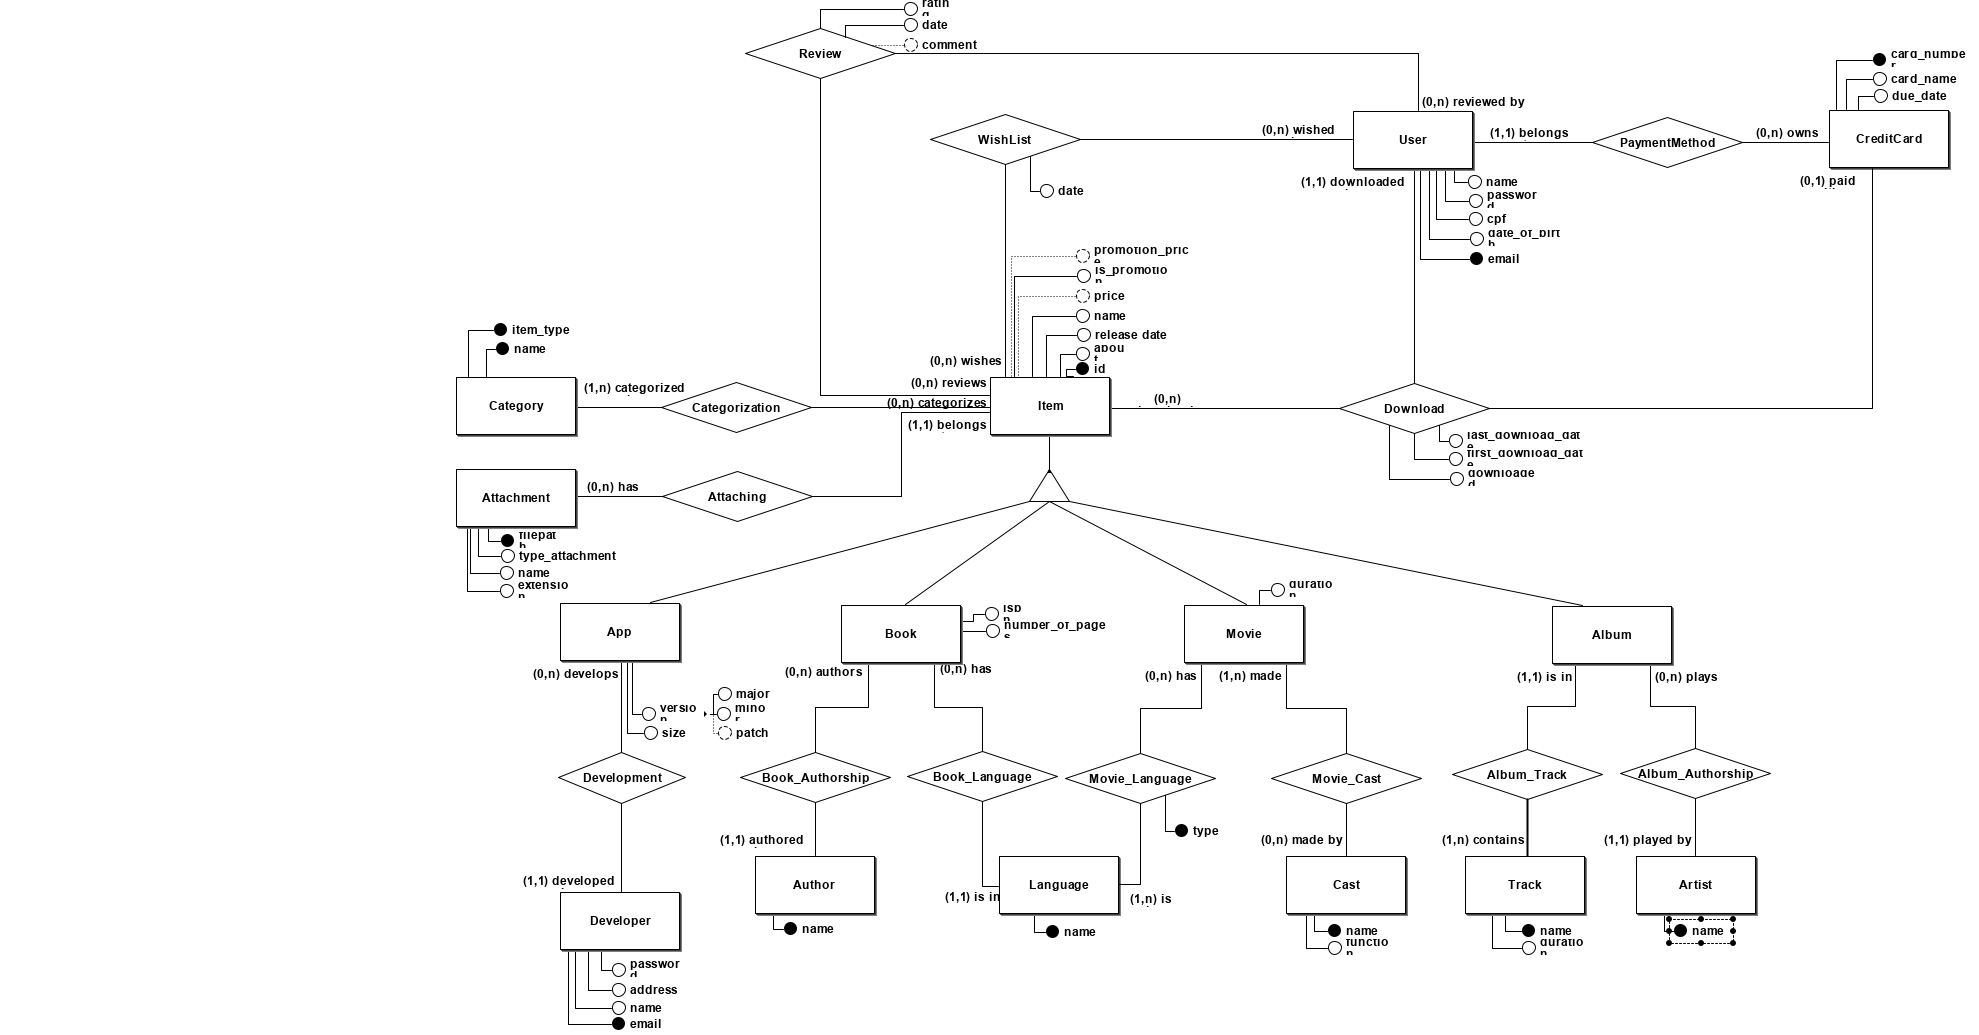
\includegraphics[angle=90, height=0.75\paperheight]{images/modeloConceitual.png}
\end{figure}

%% ===================================
\newpage
\section*{Dicionário de Dados}
O dicionário de dados será itemizado abaixo, com cada tabela representando uma entidade (ou relacionamento com atributos) presente na modelagem. Nele já transferimos o modelo conceitual para lógico, com as tabelas geradas e os atributos colocados nas posições escolhidas pelos integrantes do grupo. \\
Atributos em negrito definem que eles representam as chaves primárias das tabelas, sendo que se houver mais do que um atributo em negrito, esses atributos formam uma chave primária composta. Atributos únicos que não são definidos como chave primária (chaves candidatas) estão sublinhados. Atributos com um asterisco indicam que eles são opcionais. Todos os tipos descritos abaixos são referentes aos tipos que o PostgreSQL implementa em seu SGBD.

\vspace{1cm}

\begin{table}[h]
\centering
\resizebox{\textwidth}{!}{%
\begin{tabular}{@{}llll@{}}
\toprule
\multicolumn{4}{c}{\textbf{Item}} \\ \midrule
\multicolumn{1}{l|}{\textit{Atributo}} & \multicolumn{1}{l|}{\textit{Tipo}} &
\multicolumn{1}{l|}{\textit{Descrição}} & \textit{Exemplo} \\ \midrule
\multicolumn{1}{l|}{\textbf{id}} & \multicolumn{1}{l|}{uuid} & \multicolumn{1}{l|}{\begin{tabular}[c]{@{}l@{}}Identificador único para o item\end{tabular}} & 704ef290-... \\[10pt]
\multicolumn{1}{l|}{price*} & \multicolumn{1}{l|}{numeric(5,2)} & \multicolumn{1}{l|}{\begin{tabular}[c]{@{}l@{}}Valor a ser cobrado por um item, em reais,\\ sendo o valor limitado em R\$ 999,99.\\ Caso esse campo esteja nulo, entendemos que\\ o produto está de graça.\end{tabular}} & 9.99 \\[25pt]
\multicolumn{1}{l|}{name} & \multicolumn{1}{l|}{varchar(50)} & \multicolumn{1}{l|}{\begin{tabular}[c]{@{}l@{}}Nome do item, com no máximo\\ 50 caracteres\end{tabular}} & Super SGBD \\[15pt]
\multicolumn{1}{l|}{release\_date} & \multicolumn{1}{l|}{date} & \multicolumn{1}{l|}{Data de lançamento do item} & 31/12/2018 \\[10pt]
\multicolumn{1}{l|}{about} & \multicolumn{1}{l|}{varchar(1000)} & \multicolumn{1}{l|}{\begin{tabular}[c]{@{}l@{}}Descrição sobre o item, podendo conter\\ até no máximo 1000 caracteres\end{tabular}} & Lorem ipsum... \\[15pt]
\multicolumn{1}{l|}{is\_promotion} & \multicolumn{1}{l|}{boolean} & \multicolumn{1}{l|}{\begin{tabular}[c]{@{}l@{}}Informa se o item está ou não em promoção.\\ Se campor for true, o item é vendido pelo\\ valor descrito em promotion\_price, caso\\ contrário, é vendido pelo valor descrito em\\ price.\end{tabular}} & false \\[35pt]
\multicolumn{1}{l|}{promotion\_price*} & \multicolumn{1}{l|}{numeric(5,2)} & \multicolumn{1}{l|}{\begin{tabular}[c]{@{}l@{}}Valor a ser cobrado por um item, em reais,\\ caso o atributo is\_promotion seja true,\\ sendo o valor limitado em R\$ 999,99.\\ Caso esse campo esteja nulo, enquanto\\ is\_promotion esteja em true,\\ entendemos que o produto está de graça.\end{tabular}} &  \\[40pt]
\multicolumn{1}{l|}{type} & \multicolumn{1}{l|}{char(5)} & \multicolumn{1}{l|}{\begin{tabular}[c]{@{}l@{}}Referencia qual tipo de Item esse Item realmente é. \\ É utilizado para sabermos em qual outra tabela da\\ especificação se encontram o resto dos\\ dados (já que a generalização/especificação\\ da tabela Item é total). Pode assumir os\\ valores \{ app, movie, book, album\}\end{tabular}} & app \\\bottomrule
\end{tabular}%
}
\caption{Tabela Item e a descrição textual de seus atributos}
\end{table}

\begin{table}[]
\centering
\resizebox{\textwidth}{!}{%
\begin{tabular}{@{}llll@{}}
\toprule
\multicolumn{4}{c}{\textbf{Attachment}} \\ \midrule
\multicolumn{1}{l|}{\textit{Atributo}} & \multicolumn{1}{l|}{\textit{Tipo}} &
\multicolumn{1}{l|}{\textit{Descrição}} & \textit{Exemplo} \\ \midrule
\multicolumn{1}{l|}{\textbf{filepath}} & \multicolumn{1}{l|}{varchar(100)} & \multicolumn{1}{l|}{\begin{tabular}[c]{@{}l@{}}Caminho para onde o anexo\\ está guardado localmente\end{tabular}} & ./downloads/attach\_001.jpg \\[15pt]
\multicolumn{1}{l|}{app\_id} & \multicolumn{1}{l|}{uuid} & \multicolumn{1}{l|}{\begin{tabular}[c]{@{}l@{}}Referencia o atributo id da\\ tabela Item, para demonstrar a qual Item\\ esse Attachment pertence\end{tabular}} & 704ef290-... \\[20pt]
\multicolumn{1}{l|}{type\_attachment} & \multicolumn{1}{l|}{char(6)} & \multicolumn{1}{l|}{\begin{tabular}[c]{@{}l@{}}Tipo de anexo, sendo que os\\ possíveis valores são \{imagem, video\} \end{tabular}} & imagem \\[15pt]
\multicolumn{1}{l|}{name} & \multicolumn{1}{l|}{varchar(50)} & \multicolumn{1}{l|}{\begin{tabular}[c]{@{}l@{}}Nome dado ao anexo, para ser\\ utilizado na hora de mostrarmos\\ o mesmo na UI. \end{tabular}} & Imagem 01 \\[20pt]
\multicolumn{1}{l|}{extension} & \multicolumn{1}{l|}{char(5)} & \multicolumn{1}{l|}{\begin{tabular}[c]{@{}l@{}}Extensão dada para o arquivo \end{tabular}} & jpg \\ \bottomrule
\end{tabular}%
}
\caption{Tabela Attachment e a descrição textual de seus atributos}
\end{table}

\begin{table}[]
\centering
\resizebox{\textwidth}{!}{%
\begin{tabular}{@{}llll@{}}
\toprule
\multicolumn{4}{c}{\textbf{User}} \\ \midrule
\multicolumn{1}{l|}{\textit{Atributo}} & \multicolumn{1}{l|}{\textit{Tipo}} &
\multicolumn{1}{l|}{\textit{Descrição}} & \textit{Exemplo} \\ \midrule
\multicolumn{1}{l|}{\textbf{email}} & \multicolumn{1}{l|}{varchar(50)} & \multicolumn{1}{l|}{\begin{tabular}[c]{@{}l@{}}E-mail do usuário, válidado de\\ acordo com a RFC 5322\cite{RFC5322}\end{tabular}} & example@example.com \\[15pt]
\multicolumn{1}{l|}{name} & \multicolumn{1}{l|}{varchar(80)} & \multicolumn{1}{l|}{\begin{tabular}[c]{@{}l@{}}Nome do usuário, com no\\ máximo 80 caracteres\end{tabular}} & John Doe \\[15pt]
\multicolumn{1}{l|}{password} & \multicolumn{1}{l|}{varchar} & \multicolumn{1}{l|}{\begin{tabular}[c]{@{}l@{}}Senha do usuário, guardada com\\ criptografia SHA512\cite{SHA512}\end{tabular}} & 1253AB... \\[15pt]
\multicolumn{1}{l|}{cpf} & \multicolumn{1}{l|}{char(11)} & \multicolumn{1}{l|}{\begin{tabular}[c]{@{}l@{}}CPF do usuário, armazenado\\ sem os caracteres separadores\end{tabular}} & 99999999999 \\[15pt]
\multicolumn{1}{l|}{birthdate} & \multicolumn{1}{l|}{date} & \multicolumn{1}{l|}{\begin{tabular}[c]{@{}l@{}}Data de nascimento do usuário\end{tabular}} & 02/01/1998 \\ \bottomrule
\end{tabular}%
}
\caption{Tabela User e a descrição textual de seus atributos}
\end{table}

\begin{table}[]
\centering
\resizebox{\textwidth}{!}{%
\begin{tabular}{@{}llll@{}}
\toprule
\multicolumn{4}{c}{\textbf{Credit Card}} \\ \midrule
\multicolumn{1}{l|}{\textit{Atributo}} & \multicolumn{1}{l|}{\textit{Tipo}} &
\multicolumn{1}{l|}{\textit{Descrição}} & \textit{Exemplo} \\ \midrule
\multicolumn{1}{l|}{\textbf{card\_number}} & \multicolumn{1}{l|}{char(16)} & \multicolumn{1}{l|}{\begin{tabular}[c]{@{}l@{}}Identificador do cartão de crédito\end{tabular}} & 1111 1111 1111 1111\\[15pt]
\multicolumn{1}{l|}{user\_email} & \multicolumn{1}{l|}{varchar(50)} & \multicolumn{1}{l|}{\begin{tabular}[c]{@{}l@{}}Referencia o atributo email da\\ tabela User, para demonstral qual User\\ é o responsável por esse cartão\end{tabular}} & example@example.com\\[20pt]
\multicolumn{1}{l|}{card\_name} & \multicolumn{1}{l|}{varchar(80)} & \multicolumn{1}{l|}{\begin{tabular}[c]{@{}l@{}}Nome do dono do cartão, que pode \\ser diferente do User relacionado a\\ esse Credit Card\end{tabular}} & John Doe\\[20pt]
\multicolumn{1}{l|}{due\_date} & \multicolumn{1}{l|}{date} & \multicolumn{1}{l|}{\begin{tabular}[c]{@{}l@{}}Data de vencimento do cartão\end{tabular}} & 31/12/2025\\ \bottomrule
\end{tabular}%
}
\caption{Tabela CreditCard e a descrição textual de seus atributos}
\end{table}

\begin{table}[]
\centering
\resizebox{\textwidth}{!}{%
\begin{tabular}{@{}llll@{}}
\toprule
\multicolumn{4}{c}{\textbf{WishList}} \\ \midrule
\multicolumn{1}{l|}{\textit{Atributo}} & \multicolumn{1}{l|}{\textit{Tipo}} &
\multicolumn{1}{l|}{\textit{Descrição}} & \textit{Exemplo} \\ \midrule
\multicolumn{1}{l|}{\textbf{user\_email}} & \multicolumn{1}{l|}{varchar(50)} & \multicolumn{1}{l|}{\begin{tabular}[c]{@{}l@{}}Referencia o atributo email da tabela\\ User para demonstrar na WishList de qual\\ User o Item foi adicionado\end{tabular}} & example@example.com \\[20pt]
\multicolumn{1}{l|}{\textbf{app\_id}} & \multicolumn{1}{l|}{uuid} & \multicolumn{1}{l|}{\begin{tabular}[c]{@{}l@{}}Referencia o atributo id da\\ tabela Item, para demonstrar qual Item\\ o User adicionou em sua WishList\end{tabular}} & 704ef290-... \\[20pt]
\multicolumn{1}{l|}{date} & \multicolumn{1}{l|}{date} & \multicolumn{1}{l|}{\begin{tabular}[c]{@{}l@{}}Data na qual o Item foi adicionado\\ à WishList do User\end{tabular}} & 12/01/2019 \\ \bottomrule
\end{tabular}%
}
\caption{Tabela WishList e a descrição textual de seus atributos}
\end{table}

\begin{table}[]
\centering
\resizebox{\textwidth}{!}{%
\begin{tabular}{@{}llll@{}}
\toprule
\multicolumn{4}{c}{\textbf{Review}} \\ \midrule
\multicolumn{1}{l|}{\textit{Atributo}} & \multicolumn{1}{l|}{\textit{Tipo}} &
\multicolumn{1}{l|}{\textit{Descrição}} & \textit{Exemplo} \\ \midrule
\multicolumn{1}{l|}{\textbf{user\_email}} & \multicolumn{1}{l|}{varchar(50)} &
\multicolumn{1}{l|}{\begin{tabular}[c]{@{}l@{}}Referencia o atributo email da tabela\\ User para sabermos qual User realizou essa Review \end{tabular}} & example@example.com \\[15pt]
\multicolumn{1}{l|}{\textbf{app\_id}} & \multicolumn{1}{l|}{uuid} & \multicolumn{1}{l|}{\begin{tabular}[c]{@{}l@{}}Referencia o atributo id da\\ tabela Item, para sabermos qual Item\\ foi avaliado\end{tabular}} & 704ef290-... \\[20pt]
\multicolumn{1}{l|}{rating} & \multicolumn{1}{l|}{smallint} & \multicolumn{1}{l|}{\begin{tabular}[c]{@{}l@{}}Nota atribuída pelo User ao Item.\\ Seus valores possíveis são \{0, 1, 2, 3, 4, 5\}\end{tabular}} & 4 \\[15pt]
\multicolumn{1}{l|}{date} & \multicolumn{1}{l|}{date} & \multicolumn{1}{l|}{\begin{tabular}[c]{@{}l@{}}Data que a review aconteceu\end{tabular}} & 22/02/2019 \\[10pt]
\multicolumn{1}{l|}{comment*} & \multicolumn{1}{l|}{varchar(256)} & \multicolumn{1}{l|}{\begin{tabular}[c]{@{}l@{}}Comentário opcional do User referente ao Item\end{tabular}} & Top \\ \bottomrule
\end{tabular}%
}
\caption{Tabela Review e a descrição textual de seus atributos}
\end{table}

\begin{table}[]
\centering
\resizebox{\textwidth}{!}{%
\begin{tabular}{@{}llll@{}}
\toprule
\multicolumn{4}{c}{\textbf{Download}} \\ \midrule
\multicolumn{1}{l|}{\textit{Atributo}} & \multicolumn{1}{l|}{\textit{Tipo}} &
\multicolumn{1}{l|}{\textit{Descrição}} & \textit{Exemplo} \\ \midrule
\multicolumn{1}{l|}{\textbf{item\_id}} & \multicolumn{1}{l|}{uuid} & \multicolumn{1}{l|}{\begin{tabular}[c]{@{}l@{}}Referencia o atributo id da\\ tabela Item, para demonstrar à qual Item\\ esse download se refere\end{tabular}} & 704ef290-... \\[20pt]
\multicolumn{1}{l|}{\textbf{user\_email}} & \multicolumn{1}{l|}{varchar(50)} & \multicolumn{1}{l|}{\begin{tabular}[c]{@{}l@{}}Referencia o atributo email da\\ tabela User, para demonstrar qual User\\ realizou esse download\end{tabular}} & example@example.com \\[20pt]
\multicolumn{1}{l|}{credit\_card\_number*} & \multicolumn{1}{l|}{char(16)} & \multicolumn{1}{l|}{\begin{tabular}[c]{@{}l@{}}Referencia o atributo card\_number da\\ tabela Credit Card, para demonstrar qual\\ Credit Card o User utilizou.\\ Esse campo só está preenchido se quando o\\ User realizou o download do Item,\\ ele possuía price ou promotion\_price\\ (caso em promoção) diferente de null ou 0.\end{tabular}} & 1111 1111 1111 1111 \\[50pt]
\multicolumn{1}{l|}{first\_download\_date} & \multicolumn{1}{l|}{date} & \multicolumn{1}{l|}{\begin{tabular}[c]{@{}l@{}}Data na qual o item foi baixado pela\\ primeira vez\end{tabular}} & 18/01/2019 \\[15pt]
\multicolumn{1}{l|}{last\_download\_date} & \multicolumn{1}{l|}{date} & \multicolumn{1}{l|}{\begin{tabular}[c]{@{}l@{}}Data na qual o item foi baixado pela\\ última vez. É sempre maior ou igual a\\ first\_download\_date.\end{tabular}} & 18/01/2019 \\[20pt]
\multicolumn{1}{l|}{downloaded} & \multicolumn{1}{l|}{boolean} & \multicolumn{1}{l|}{\begin{tabular}[c]{@{}l@{}}Informa se o item está instalado (true)\\ ou desinstalado (false) no momento\end{tabular}} & false \\ \bottomrule
\end{tabular}%
}\caption{Tabela Download e a descrição textual de seus atributos}
\end{table}

\begin{table}[]
\centering
\resizebox{\textwidth}{!}{%
\begin{tabular}{@{}llll@{}}
\toprule
\multicolumn{4}{c}{\textbf{Language}} \\ \midrule
\multicolumn{1}{l|}{\textit{Atributo}} & \multicolumn{1}{l|}{\textit{Tipo}} &
\multicolumn{1}{l|}{\textit{Descrição}} & \textit{Exemplo} \\ \midrule
\multicolumn{1}{l|}{\textbf{name}} & \multicolumn{1}{l|}{varchar(20)} & \multicolumn{1}{l|}{\begin{tabular}[c]{@{}l@{}}Nome da linguagem, com no máximo\\ 20 caracteres\end{tabular}} & italiano \\ \bottomrule
\end{tabular}%
}
\caption{Tabela Language e a descrição textual de seus atributos}
\end{table}

\begin{table}[]
\centering
\resizebox{\textwidth}{!}{%
\begin{tabular}{@{}llll@{}}
\toprule
\multicolumn{4}{c}{\textbf{Developer}} \\ \midrule
\multicolumn{1}{l|}{\textit{Atributo}} & \multicolumn{1}{l|}{\textit{Tipo}} &
\multicolumn{1}{l|}{\textit{Descrição}} & \textit{Exemplo} \\ \midrule
\multicolumn{1}{l|}{\textbf{email}} & \multicolumn{1}{l|}{varchar(50)} & \multicolumn{1}{l|}{\begin{tabular}[c]{@{}l@{}}E-mail do(a) desenvolvedor(a),\\ validado de acordo com a RFC 5322\cite{RFC5322}\end{tabular}} & developer@example.com \\[15pt]
\multicolumn{1}{l|}{name} & \multicolumn{1}{l|}{varchar(80)} & \multicolumn{1}{l|}{\begin{tabular}[c]{@{}l@{}}Nome do(a) desenvolvedor(a),\\ com no máximo 80 caracteres\end{tabular}} & Developer Doe \\[15pt]
\multicolumn{1}{l|}{address} & \multicolumn{1}{l|}{varchar} & \multicolumn{1}{l|}{\begin{tabular}[c]{@{}l@{}}Endereço do(a) desenvolvedor(a)\\ contendo rua, número, bairro, cidade\\ e país, ou conforme for o padrão do país\\ de origem do(a) desenvolvedor(a) \end{tabular}} & ..., Havana, Cuba \\[25pt]
\multicolumn{1}{l|}{password} & \multicolumn{1}{l|}{varchar} & \multicolumn{1}{l|}{\begin{tabular}[c]{@{}l@{}}Senha do developer, guardada com\\ criptografia SHA512\cite{SHA512} \end{tabular}} & 8269bf0a... \\\bottomrule
\end{tabular}%
}
\caption{Tabela Developer e a descrição textual de seus atributos}
\end{table}

\begin{table}[]
\centering
\resizebox{\textwidth}{!}{%
\begin{tabular}{@{}llll@{}}
\toprule
\multicolumn{4}{c}{\textbf{Artist}} \\ \midrule
\multicolumn{1}{l|}{\textit{Atributo}} & \multicolumn{1}{l|}{\textit{Tipo}} &
\multicolumn{1}{l|}{\textit{Descrição}} & \textit{Exemplo} \\ \midrule
\multicolumn{1}{l|}{\textbf{name}} & \multicolumn{1}{l|}{varchar(80)} & \multicolumn{1}{l|}{\begin{tabular}[c]{@{}l@{}}Representa o nome de um artista que pode possuir algum Album.\\ Nome pode possuir no máximo 80 caracteres\end{tabular}} & Artist Doe \\ \bottomrule
\end{tabular}%
}
\caption{Tabela Artist e a descrição textual de seus atributos}
\end{table}


\begin{table}[]
\centering
\resizebox{\textwidth}{!}{%
\begin{tabular}{@{}llll@{}}
\toprule
\multicolumn{4}{c}{\textbf{Author}} \\ \midrule
\multicolumn{1}{l|}{\textit{Atributo}} & \multicolumn{1}{l|}{\textit{Tipo}} &
\multicolumn{1}{l|}{\textit{Descrição}} & \textit{Exemplo} \\ \midrule
\multicolumn{1}{l|}{\textbf{name}} & \multicolumn{1}{l|}{varchar(80)} & \multicolumn{1}{l|}{\begin{tabular}[c]{@{}l@{}}Nome do autor, com no máximo\\ 80 caracteres\end{tabular}} & Author Doe \\ \bottomrule
\end{tabular}%
}
\caption{Tabela Author e a descrição textual de seus atributos}
\end{table}

\begin{table}[]
\centering
\resizebox{\textwidth}{!}{%
\begin{tabular}{@{}llll@{}}
\toprule
\multicolumn{4}{c}{\textbf{Cast}} \\ \midrule
\multicolumn{1}{l|}{\textit{Atributo}} & \multicolumn{1}{l|}{\textit{Tipo}} &
\multicolumn{1}{l|}{\textit{Descrição}} & \textit{Exemplo} \\ \midrule
\multicolumn{1}{l|}{\textbf{name}} & \multicolumn{1}{l|}{varchar(80)} & \multicolumn{1}{l|}{\begin{tabular}[c]{@{}l@{}}Nome da pessoa que pertence ao Cast\\ de algum filme\end{tabular}} & Cast Doe \\[15pt]
\multicolumn{1}{l|}{function} & \multicolumn{1}{l|}{char(8)} & \multicolumn{1}{l|}{\begin{tabular}[c]{@{}l@{}}Função que a pessoa desempenhou no filme.\\ É um dos valores entre \{actor, director, producer, writer\}\end{tabular}} & writer \\ \bottomrule
\end{tabular}%
}
\caption{Tabela Cast e a descrição textual de seus atributos}
\end{table}

\begin{table}[]
\centering
\resizebox{\textwidth}{!}{%
\begin{tabular}{@{}llll@{}}
\toprule
\multicolumn{4}{c}{\textbf{Category}} \\ \midrule
\multicolumn{1}{l|}{\textit{Atributo}} & \multicolumn{1}{l|}{\textit{Tipo}} &
\multicolumn{1}{l|}{\textit{Descrição}} & \textit{Exemplo} \\ \midrule
\multicolumn{1}{l|}{\textbf{name}} & \multicolumn{1}{l|}{varchar(25)} & \multicolumn{1}{l|}{\begin{tabular}[c]{@{}l@{}}Nome da categoria, sendo único\\ dentro do mesmo item\_type\end{tabular}} & Ficção Científica \\[15pt]
\multicolumn{1}{l|}{\textbf{item\_type}} & \multicolumn{1}{l|}{char(5)} & \multicolumn{1}{l|}{\begin{tabular}[c]{@{}l@{}}Tipo de item à qual essa categoria\\ se aplica. Os valores possíveis são\\ \{app, livro, filme, album\}. Para o\\ mesmo item\_type, não podem haver 2\\ categorias com o mesmo nome. \\ Isso significa que item\_type e name \\ \textbf{juntos}, identificam uma categoria.\end{tabular}} & filme \\ \bottomrule
\end{tabular}%
}
\caption{Tabela Category e a descrição textual de seus atributos. Mais informações sobre ela na Tabela 2.}
\end{table}

\begin{table}[]
\centering
\resizebox{\textwidth}{!}{%
\begin{tabular}{@{}llll@{}}
\toprule
\multicolumn{4}{c}{\textbf{Categorization}} \\ \midrule
\multicolumn{1}{l|}{\textit{Atributo}} & \multicolumn{1}{l|}{\textit{Tipo}} &
\multicolumn{1}{l|}{\textit{Descrição}} & \textit{Exemplo} \\ \midrule
\multicolumn{1}{l|}{\textbf{category\_name}} & \multicolumn{1}{l|}{varchar(25)} & \multicolumn{1}{l|}{\begin{tabular}[c]{@{}l@{}}Referencia o atributo name da tabela\\ Category, associando essa Categoria a um Item\end{tabular}} & Ficção Científica \\[15pt]
\multicolumn{1}{l|}{\textbf{category\_item\_type}} & \multicolumn{1}{l|}{char(5)} & \multicolumn{1}{l|}{\begin{tabular}[c]{@{}l@{}}Referencia o atributo item\_type da tabela\\ Category, informando a qual tipo de Item\\ essa categoria pode se relacionar.\\ O Item referenciado por essa Categorization\\ precisa ser do mesmo tipo que o descrito\\ nesse campo.\end{tabular}} & filme \\[35pt]
\multicolumn{1}{l|}{\textbf{item\_id}} & \multicolumn{1}{l|}{uuid} & \multicolumn{1}{l|}{\begin{tabular}[c]{@{}l@{}}Referencia o atributo id da tabela\\ Item, fazendo com que uma Category\\ seja associada a um Item.\end{tabular}} & 704ef290-... \\ \bottomrule
\end{tabular}%
}
\caption{Tabela Categorization e a descrição textual de seus atributos}
\end{table}

\begin{table}[]
\centering
\resizebox{\textwidth}{!}{%
\begin{tabular}{@{}llll@{}}
\toprule
\multicolumn{4}{c}{\textbf{App \textit{(que especifica a tabela Item)}}} \\ \midrule
\multicolumn{1}{l|}{\textit{Atributo}} & \multicolumn{1}{l|}{\textit{Tipo}} &
\multicolumn{1}{l|}{\textit{Descrição}} & \textit{Exemplo} \\ \midrule
\multicolumn{1}{l|}{\textbf{app\_id}} & \multicolumn{1}{l|}{uuid} & \multicolumn{1}{l|}{\begin{tabular}[c]{@{}l@{}}Referencia o atributo id da\\ tabela Item, para encontramos os dados\\ adicionais referentes ao App\end{tabular}} & 704ef290-... \\[20pt]
\multicolumn{1}{l|}{developer\_email} & \multicolumn{1}{l|}{varchar(50)} & \multicolumn{1}{l|}{\begin{tabular}[c]{@{}l@{}}Referencia o atributo email da\\ tabela Developer, para sabermos quem\\ foi o(a) desenvolvedor(a) desse App\end{tabular}} & developer@example.com \\[20pt]
\multicolumn{1}{l|}{size} & \multicolumn{1}{l|}{bigint} & \multicolumn{1}{l|}{\begin{tabular}[c]{@{}l@{}}Tamanho do aplicativo, em bytes\end{tabular}} & 1048576 \\[15pt]
\multicolumn{1}{l|}{version} & \multicolumn{1}{l|}{varchar} & \multicolumn{1}{l|}{\begin{tabular}[c]{@{}l@{}}Texto demonstrando a versão do app no formato\\ "MAJOR.MINOR.PATCH", sendo que MAJOR, MINOR\\ e PATCH são números inteiros, sem vírgulas, e PATCH\\ pode ser omitido juntamente com o ponto anterior à ele \end{tabular}} & 2.1.12 \\ \bottomrule
\end{tabular}%
}
\caption{Tabela App (que especifica a tabela Item) e a descrição textual de seus atributos}
\end{table}

\begin{table}[]
\centering
\resizebox{\textwidth}{!}{%
\begin{tabular}{@{}llll@{}}
\toprule
\multicolumn{4}{c}{\textbf{Album \textit{(que especifica a tabela Item)}}} \\ \midrule
\multicolumn{1}{l|}{\textit{Atributo}} & \multicolumn{1}{l|}{\textit{Tipo}} &
\multicolumn{1}{l|}{\textit{Descrição}} & \textit{Exemplo} \\ \midrule
\multicolumn{1}{l|}{\textbf{app\_id}} & \multicolumn{1}{l|}{uuid} & \multicolumn{1}{l|}{\begin{tabular}[c]{@{}l@{}}Referencia o atributo id da\\ tabela Item, para encontramos os dados\\ adicionais referentes ao Album\end{tabular}} & 704ef290-... \\[20pt]
\multicolumn{1}{l|}{\textbf{artist\_name}} & \multicolumn{1}{l|}{varchar(80)} & \multicolumn{1}{l|}{\begin{tabular}[c]{@{}l@{}}Referencia o atributo name da\\ tabela Arist, para encontramos o\\ cantor/produtor desse album\end{tabular}} & Artist Doe \\ \bottomrule
\end{tabular}%
}
\caption{Tabela Album (que especifica a tabela Item) e a descrição textual de seus atributos}
\end{table}

\begin{table}[]
\centering
\resizebox{\textwidth}{!}{%
\begin{tabular}{@{}llll@{}}
\toprule
\multicolumn{4}{c}{\textbf{Track}} \\ \midrule
\multicolumn{1}{l|}{\textit{Atributo}} & \multicolumn{1}{l|}{\textit{Tipo}} &
\multicolumn{1}{l|}{\textit{Descrição}} & \textit{Exemplo} \\ \midrule
\multicolumn{1}{l|}{\textbf{album\_id}} & \multicolumn{1}{l|}{uuid} & \multicolumn{1}{l|}{\begin{tabular}[c]{@{}l@{}}Referencia o atributo app\_id da\\ tabela Album, para sabermos de qual Album\\ essa música pertence\end{tabular}} & 704ef290-... \\[20pt]
\multicolumn{1}{l|}{\textbf{name}} & \multicolumn{1}{l|}{varchar(50)} & \multicolumn{1}{l|}{\begin{tabular}[c]{@{}l@{}}Nome da música, sendo única dentro de um álbum.\\ Possui no máximo 50 caracteres\end{tabular}} & Juntos e Shallow Now \\[15pt]
\multicolumn{1}{l|}{duration} & \multicolumn{1}{l|}{int} & \multicolumn{1}{l|}{\begin{tabular}[c]{@{}l@{}}Duração da música em segundos\end{tabular}} & 205 \\\bottomrule
\end{tabular}%
}
\caption{Tabela Track e a descrição textual de seus atributos}
\end{table}

\begin{table}[]
\centering
\resizebox{\textwidth}{!}{%
\begin{tabular}{@{}llll@{}}
\toprule
\multicolumn{4}{c}{\textbf{Book \textit{(que especifica a tabela Item)}}} \\ \midrule
\multicolumn{1}{l|}{\textit{Atributo}} & \multicolumn{1}{l|}{\textit{Tipo}} &
\multicolumn{1}{l|}{\textit{Descrição}} & \textit{Exemplo} \\ \midrule
\multicolumn{1}{l|}{\textbf{item\_id}} & \multicolumn{1}{l|}{uuid} & \multicolumn{1}{l|}{\begin{tabular}[c]{@{}l@{}}Referencia o atributo id da\\ tabela Item, para encontramos os dados\\ adicionais referentes ao Book\end{tabular}} & 704ef290-... \\[20pt]
\multicolumn{1}{l|}{author\_name} & \multicolumn{1}{l|}{varchar(80)} & \multicolumn{1}{l|}{\begin{tabular}[c]{@{}l@{}}Referencia o atributo name da\\ tabela Author, para sabermos quem\\ foi o(a) autor(a) desse Book\end{tabular}} & Author Doe \\[20pt]
\multicolumn{1}{l|}{language\_name} & \multicolumn{1}{l|}{varchar(80)} & \multicolumn{1}{l|}{\begin{tabular}[c]{@{}l@{}}Referencia o atributo name da\\ tabela Language, para sabermos em qual\\ linguagem o livro está escrito\end{tabular}} & Italiano \\[20pt]
\multicolumn{1}{l|}{number\_of\_pages} & \multicolumn{1}{l|}{smallint} & \multicolumn{1}{l|}{\begin{tabular}[c]{@{}l@{}}Quantidade de páginas no livro\end{tabular}} & 425 \\[10pt]
\multicolumn{1}{l|}{\underline{ISBN}} & \multicolumn{1}{l|}{char(13)} & \multicolumn{1}{l|}{\begin{tabular}[c]{@{}l@{}}ISBN (código identificador) do livro\cite{ISBN}\end{tabular}} & 9788533302273 \\ \bottomrule
\end{tabular}%
}
\caption{Tabela Book (que especifica a tabela Item) e a descrição textual de seus atributos}
\end{table}


\begin{table}[]
\centering
\resizebox{\textwidth}{!}{%
\begin{tabular}{@{}llll@{}}
\toprule
\multicolumn{4}{c}{\textbf{Movie \textit{(que especifica a tabela Item)}}} \\ \midrule
\multicolumn{1}{l|}{\textit{Atributo}} & \multicolumn{1}{l|}{\textit{Tipo}} &
\multicolumn{1}{l|}{\textit{Descrição}} & \textit{Exemplo} \\ \midrule
\multicolumn{1}{l|}{\textbf{app\_id}} & \multicolumn{1}{l|}{uuid} & \multicolumn{1}{l|}{\begin{tabular}[c]{@{}l@{}}Referencia o atributo id da tabela Item,\\ para encontramos os dados adicionais referentes\\ ao Movie\end{tabular}} & 704ef290-... \\[20pt]
\multicolumn{1}{l|}{duration} & \multicolumn{1}{l|}{int} & \multicolumn{1}{l|}{\begin{tabular}[c]{@{}l@{}}Quantidade de minutos do filme\end{tabular}} & 123 \\ \bottomrule
\end{tabular}%
}
\caption{Tabela Movie (que especifica a tabela Item) e a descrição textual de seus atributos}
\end{table}

\begin{table}[]
\centering
\resizebox{\textwidth}{!}{%
\begin{tabular}{@{}llll@{}}
\toprule
\multicolumn{4}{c}{\textbf{Movie\_Language}} \\ \midrule
\multicolumn{1}{l|}{\textit{Atributo}} & \multicolumn{1}{l|}{\textit{Tipo}} &
\multicolumn{1}{l|}{\textit{Descrição}} & \textit{Exemplo} \\ \midrule
\multicolumn{1}{l|}{\textbf{movie\_id}} & \multicolumn{1}{l|}{uuid} & \multicolumn{1}{l|}{\begin{tabular}[c]{@{}l@{}}Referencia o atributo app\_id da\\ tabela Movie, para sabermos qual filme\\ possui essa linguagem\end{tabular}} & 704ef290-... \\[20pt]
\multicolumn{1}{l|}{\textbf{language\_name}} & \multicolumn{1}{l|}{varchar(80)} & \multicolumn{1}{l|}{\begin{tabular}[c]{@{}l@{}}Referencia o atributo name da\\ tabela Language, para sabermos qual\\ linguagem o filme indicado em movie\_id possui\end{tabular}} & Italiano \\[20pt]
\multicolumn{1}{l|}{\textbf{type}} & \multicolumn{1}{l|}{char(7)} & \multicolumn{1}{l|}{\begin{tabular}[c]{@{}l@{}}Representa se essa linguagem para esse filme\\ é relacionada à legenda ou ao áudio.\\ Os únicos valores permitidos são \{audio, legenda\}\end{tabular}} & legenda \\ \bottomrule
\end{tabular}%
}
\caption{Tabela Movie\_Language e a descrição textual de seus atributos}
\end{table}

\begin{table}[]
\centering
\resizebox{\textwidth}{!}{%
\begin{tabular}{@{}llll@{}}
\toprule
\multicolumn{4}{c}{\textbf{Movie\_Cast}} \\ \midrule
\multicolumn{1}{l|}{\textit{Atributo}} & \multicolumn{1}{l|}{\textit{Tipo}} &
\multicolumn{1}{l|}{\textit{Descrição}} & \textit{Exemplo} \\ \midrule
\multicolumn{1}{l|}{\textbf{movie\_id}} & \multicolumn{1}{l|}{uuid} & \multicolumn{1}{l|}{\begin{tabular}[c]{@{}l@{}}Referencia o atributo app\_id da\\ tabela Movie, para sabermos qual filme\\ possui essa pessoa no Cast\end{tabular}} & 704ef290-... \\[20pt]
\multicolumn{1}{l|}{\textbf{cast\_name}} & \multicolumn{1}{l|}{varchar(80)} & \multicolumn{1}{l|}{\begin{tabular}[c]{@{}l@{}}Referencia o atributo name da\\ tabela Cast, para sabermos qual\\ pessoa do cast participou do filme indicado em movie\_id\end{tabular}} & Cast Doe \\ \bottomrule
\end{tabular}%
}
\caption{Tabela Movie\_Cast e a descrição textual de seus atributos}
\end{table}

%% ===================================
\clearpage
\section*{Modelo Lógico}
\begin{figure}[H]
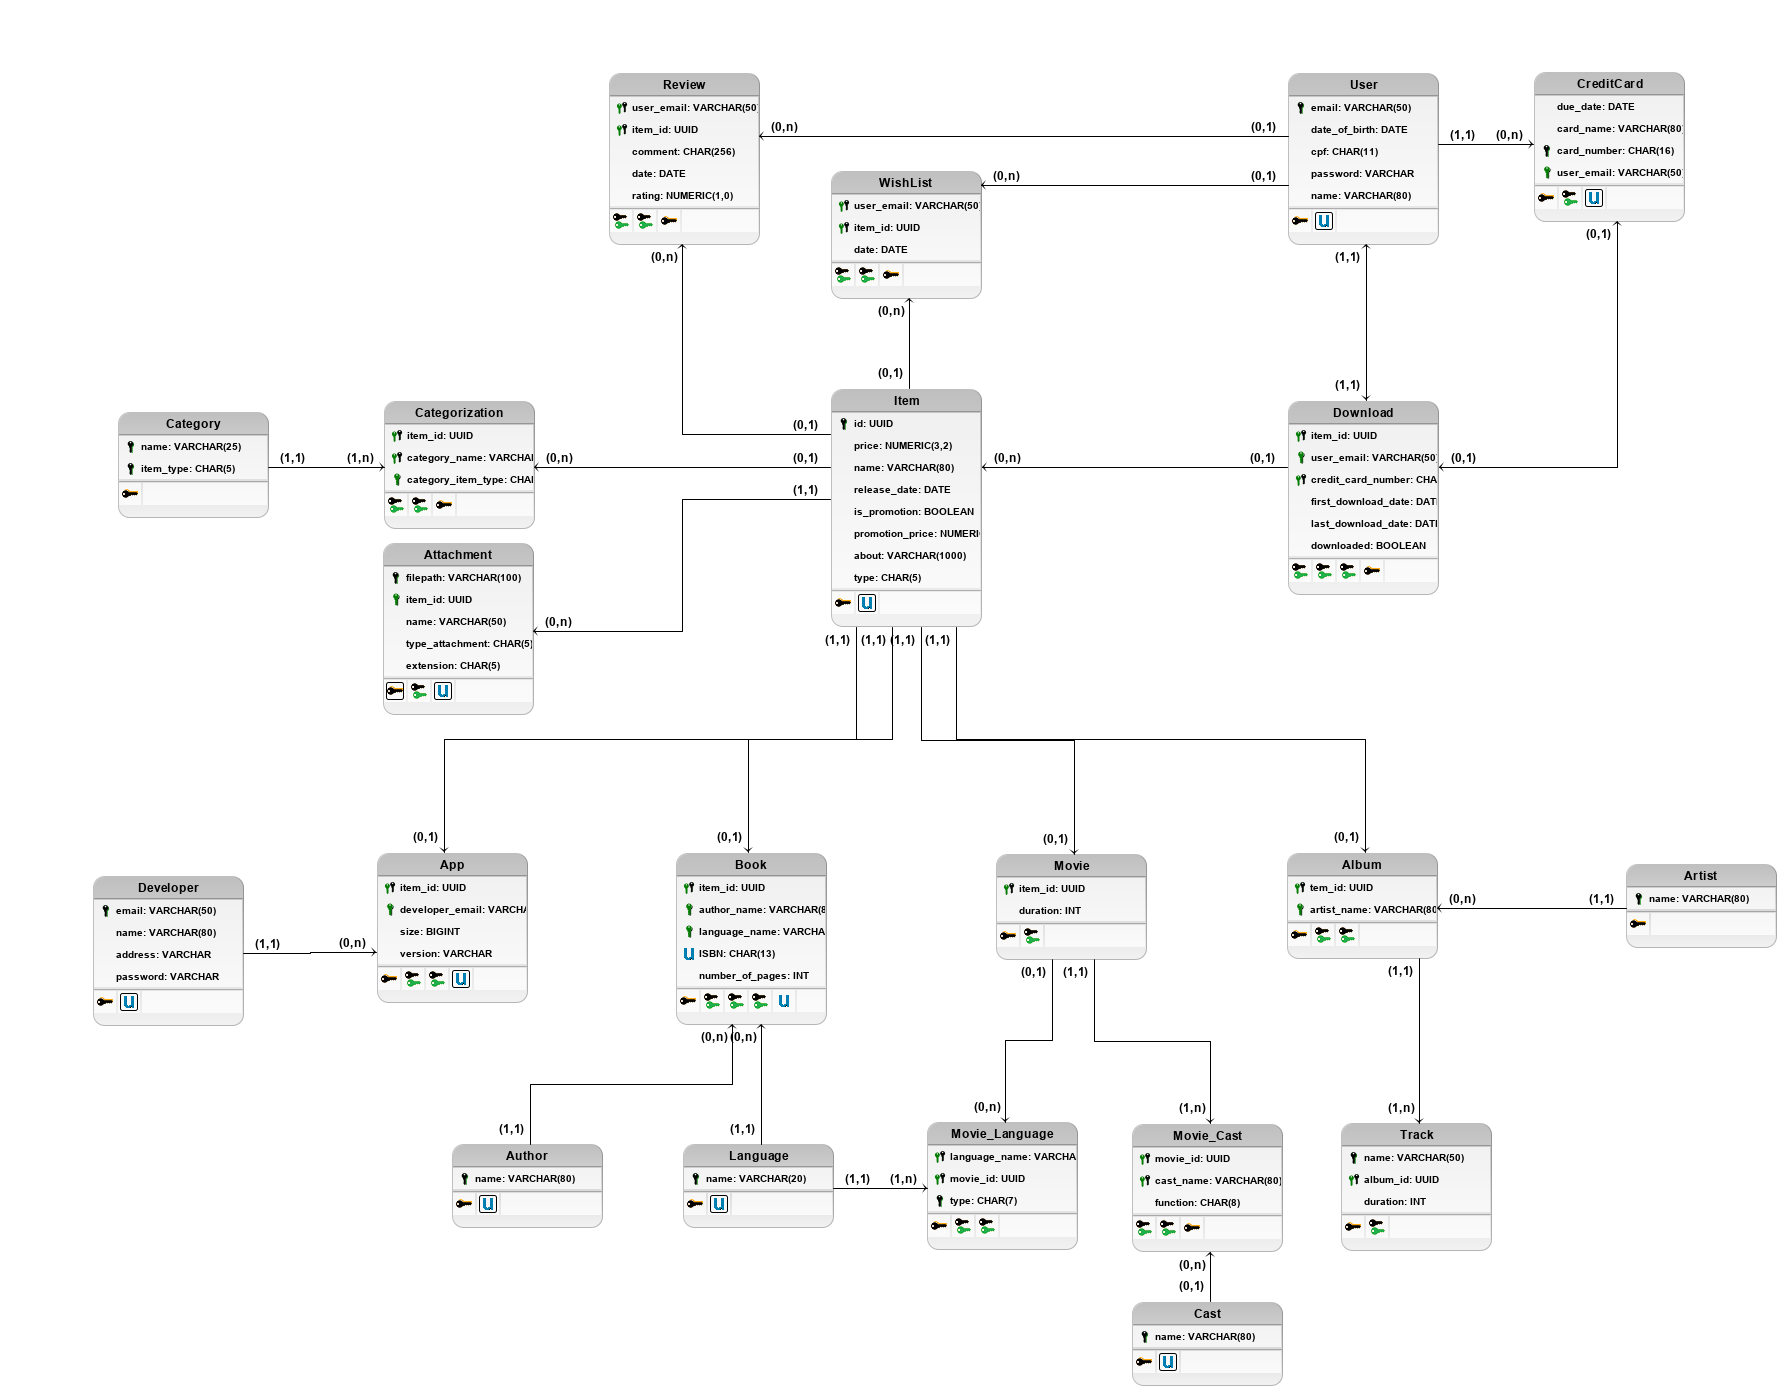
\includegraphics[angle=90, height=0.75\paperheight]{images/modeloRelacional.png}
\end{figure}

%% ===================================
\newpage
\section*{Descrição do Mapeamento (Conceitual para Lógico)}

Segue uma lista de mapeamentos implementados, onde os atributos, entidades e relacionamentos que estão escritos com  itálico, são campos adicionais que não estavam no modelo conceitual e os que são definidos como "Mapeamento direto" querem dizer que estão da mesma maneira como foram definidos no conceitual.

Entidades:
\begin{itemize}
    \item User: Mapeamento direto para {\textbf{User}}.
    \begin{itemize}
        \item name: Mapeamento direto para {\textbf{User.name}}, obrigatório.
        \item email: Mapeamento direto para {\textbf{User.email}}, obrigatório e chave primária.
        \item date\_of\_birth: Mapeamento direto para {\textbf{User.date\_of\_birth}}, obrigatório.
        \item password: Mapeamento direto para {\textbf{User.password}}, obrigatório.
    \end{itemize}
    \item CreditCard: Mapeamento direto para {\textbf{CreditCard}}.
    \begin{itemize}
        \item due\_date: Mapeamento direto para {\textbf{CreditCard.due\_date}}, obrigatório.
        \item card\_name: Mapeamento direto para {\textbf{CreditCard.card\_name}}, obrigatório.
        \item card\_number: Mapeamento direto para {\textbf{CreditCard.card\_number}}, obrigatório e chave primária.
        \item{\textit{user\_email}}: Identificador do usuário, por conta do mapeamento de relacionamento por colunas adicionais no relacionamento PaymentMethod. Mapeado para {\textbf{CreditCard.user\_email}}, obrigatório e chave estrangeira.
    \end{itemize}
    \item Item: Como é uma generalização total e exclusiva, o mapeamento foi feito seguindo a alternativa 1 (segundo os slides de mapeamento). Onde foi usada como chave estrangeira (única) na entidade especializada a chave primária da entidade generalizada, fazendo com que sempre que ocorre uma entidade especializada, exista uma entidade generalizada que ainda não foi relacionada. Mapeada para {\textbf{Item}}.
    \begin{itemize}
        \item {\textit{id}}: É um índice criado para ser a chave primária do item, pois como não existe nenhum atributo sozinho que é único, e ele tem que ser usado como chave estrangeira na entidade especializada, foi decidido que seria lógico usar um índice, por conta do menor espaço ocupado e facilidade. Mapeado para  {\textbf{Item.id}}, obrigatório e chave primária, sendo do tipo UUID, automaticamente gerado pelo banco de dados.
        \item name: Mapeamento direto para {\textbf{Item.name}}, obrigatório.
        \item price: Mapeamento direto para {\textbf{Item.price}}, opcional.
        \item release\_date: Mapeamento direto para {\textbf{Item.release\_date}}, obrigatório.
        \item is\_promotion: Mapeamento direto para {\textbf{Item.is\_promotion}}, obrigatório.
        \item promotion\_price: Mapeamento direto para {\textbf{Item.promotion\_price}}, opcional.
        \item about: Mapeamento direto para {\textbf{Item.about}}, obrigatório.
    \end{itemize}
    \item App: Entidade especializada de item, onde contém como chave primária, uma chave estrangeira para item, fazendo com que seja obrigatória a existência do mesmo para sua criação. Mapeada para {\textbf{App}}.
    \begin{itemize}
        \item {\textit{item\_id}}: É uma chave estrangeira para Item, ao mesmo tempo em que é chave primária, fazendo com que seja único o relacionamento com Item e não exista nenhum outro App relacionado com o mesmo. Mapeamento direto para {\textbf{App.item\_id}}, obrigatório e chave primária.
        \item {\textit{developer\_email}}: É uma chave estrangeira para Developer. Mapeado para {\textbf{App. developer\_email}}, obrigatório.
        \item size: Mapeamento direto para {\textbf{App.size}}, obrigatório.
        \item version: Mapeamento direto para {\textbf{App.version}}, obrigatório.
    \end{itemize}
    \item Book: Entidade especializada de item, onde contém como chave primária, uma chave estrangeira para item, fazendo com que seja obrigatória a existência do mesmo para sua criação. Mapeada para {\textbf{Book}}.
    \begin{itemize}
        \item {\textit{item\_id}}: É uma chave estrangeira para Item, ao mesmo tempo em que é chave primária, fazendo com que seja único o relacionamento com Item e não exista nenhum outro App relacionado com o mesmo. Mapeamento direto para {\textbf{Book.item\_id}}, obrigatório e chave primária.
        \item {\textit{author\_name}}: Chave estrangeira para a tabela Author. Mapeado para {\textbf{Book. author\_name}}, obrigatório.
        \item {\textit{language\_name}}: Chave estrangeira para a tabela Language. Mapeado para {\textbf{Book. language\_name}}, obrigatório.
        \item isbn: Mapeamento direto para {\textbf{Book.isbn}}, obrigatório e único.
        \item number\_of\_pages: Mapeamento direto para {\textbf{Book.number\_of\_pages}}, obrigatório.
    \end{itemize}
    \item Movie: Entidade especializada de item, onde contém como chave primária, uma chave estrangeira para item, fazendo com que seja obrigatória a existência do mesmo para sua criação. Mapeada para {\textbf{Movie}}.
    \begin{itemize}
        \item {\textit{item\_id}}: É uma chave estrangeira para Item, ao mesmo tempo em que é chave primária, fazendo com que seja único o relacionamento com Item e não exista nenhum outro App relacionado com o mesmo. Mapeamento direto para {\textbf{Movie.item\_id}}, obrigatório e chave primária.
        \item duraration: Mapeamento direto para {\textbf{Movie.duration}}, obrigatório.
    \end{itemize}
    \item Album: Entidade especializada de item, onde contém como chave primária, uma chave estrangeira para item, fazendo com que seja obrigatória a existência do mesmo para sua criação. Mapeada para {\textbf{Album}}.
    \begin{itemize}
        \item {\textit{item\_id}}: É uma chave estrangeira para Item, ao mesmo tempo em que é chave primária, fazendo com que seja único o relacionamento com Item e não exista nenhum outro App relacionado com o mesmo. Mapeamento direto para {\textbf{Album.item\_id}}, obrigatório e chave primária.
        \item {\textit{artist\_name}}: É uma chave estrangeira para Album. Mapeado para {\textbf{Album. artist\_name}}, obrigatório.
    \end{itemize}
    \item Developer: Mapeamento direto para {\textbf{Developer}}.
    \begin{itemize}
        \item email: Mapeamento direto para {\textbf{Developer.email}}, obrigatório e chave primária, pois é a única chave candidata.
        \item name: Mapeamento direto para {\textbf{developer.name}}, obrigatório.
        \item address: Mapeamento direto para {\textbf{Developer.address}}, obrigatório.
        \item password: Mapeamento direto para {\textbf{Developer.password}}, obrigatório.
    \end{itemize}
    \item Author: Mapeamento direto para {\textbf{Author}}.
    \begin{itemize}
        \item name: Mapeamento direto para {\textbf{Author.name}}, obrigatório e chave primária, pois é a única chave candidata, além de ser o único atributo.
    \end{itemize}
    \item Language: Mapeamento direto para {\textbf{Language}}.
    \begin{itemize}
        \item name: Mapeamento direto para {\textbf{Language.name}}, obrigatório e chave primária, pois é a única chave candidat, além de ser o único atributoa.
    \end{itemize}
    \item Cast: Mapeamento direto para {\textbf{Cast}}.
    \begin{itemize}
        \item name: Mapeamento direto para {\textbf{Cast.name}}, obrigatório e chave primária, pois é a única chave candidata, além de ser o único atributo.
    \end{itemize}
    \item Track: Mapeamento direto para {\textbf{Track}}.
    \begin{itemize}
        \item name: Mapeamento direto para {\textbf{Track.name}}, obrigatório e chave primária juntamente com \textbf{Track.album\_id}, já que \textbf{Track} é uma entidade fraca.
        \item \textit{album\_id}: Mapeamento direto para {\textbf{Track.album\_id}}, obrigatório e chave primária juntamente com \textbf{Track.name}, já que \textbf{Track} é uma entidade fraca em relação a \textbf{Album}.
        \item duration: Mapeamento direto para {\textbf{Track.duration}}, obrigatório e não nulo.
    \end{itemize}
    \item Attachment: Mapeamento direto para {\textbf{Attachment}}
    \begin{itemize}
        \item filepath: Mapeamento direto para \textbf{Attachment.filepath}, obrigatório e não nulo, é a chave primária da tabela por ser a única chave candidata.
        \item \textit{item\_id}: Mapeamento direto para \textbf{Attachment.item\_id}, obrigatório e não nulo, é uma chave estrangeira para a tabela Item, representando o relacionamento Attaching.
        \item name: Mapeamento direto para \textbf{Attachment.name}, obrigatório e não nulo.
        \item type\_attachment: Mapeamento direto para \textbf{Attachment.type\_attachment}, obrigatório e não nulo.
        \item extension: Mapeamento direto para \textbf{Attachment.extension}, obrigatório e não nulo.
    \end{itemize}
    \item Category: Mapeamento direto para {\textbf{Category}}
    \begin{itemize}
        \item name: Mapeamento direto para \textbf{Category.name}, obrigatório e não nulo, é unico juntamente com \textbf{Category.item\_type}, assim como chave primária juntamente com ele. 
        \item item\_type:Mapeamento direto para \textbf{Category.item\_type}, obrigatório e não nulo, é unico juntamente com \textbf{Category.name}, assim como chave primária, juntamente com ele.
    \end{itemize}
\end{itemize}
\break
Relacionamentos:
\begin{itemize}
    \item PaymentMethod: Mapeamento de relacionamento por colunas adicionais, pois é um relacionamento $1$:$N$. Com a chave estrangeira em CreditCard.
    \item Review: Mapeamento de relacionamento por tabela própria, pois é um relacionamento $N$:$M$.
    \begin{itemize}
        \item {\textit{user\_email}}: Chave primária do usuário, por ser uma tabela de relação que liga usuário a itens. Mapeado para {\textbf{Review.user\_email}}, obrigatório e chave estrangeira.
        \item {\textit{item\_id}}: Chave primária do item, pelo mesmo motivo do atributo user\_email. Mapeado para {\textbf{Review.item\_id}}, obrigatório e chave estrangeira.
        \item comment: Mapeamento direto para {\textbf{Review.comment}}, opcional.
        \item date: Mapeamento direto para {\textbf{Review.date}}, obrigatório.
        \item rating: Mapeamento direto para {\textbf{Review.rating}}, obrigatório.
    \end{itemize}
    \item WishList: Mapeamento de relacionamento por tabela própria, pois é um relacionamento $N$:$M$. 
    \begin{itemize}
        \item {\textit{user\_email}}: Chave primária do usuário, por ser uma tabela de relação que liga usuário a itens. Mapeado para {\textbf{WhishList.user\_email}}, obrigatório e chave estrangeira.
        \item {\textit{item\_id}}: Chave primária do item, pelo mesmo motivo do atributo user\_email. Mapeado para {\textbf{WishList.item\_id}}, obrigatório e chave estrangeira.
        \item date: Mapeamento direto para  {\textbf{WhishList.date}}, obrigatório.
    \end{itemize}
    \item Download: Mapeamento de relacionamento por tabela própria, pois é um relacionamento ternário. Foi implementada uma tabela com referência (chave estrangeira) às chaves primárias de User, CreditCart e Item.
    \begin{itemize}
        \item {\textit{item\_id}}: Chave primária do item, que está fazendo parte da chave composta que identifica o prórpio Download. Mapeado para {\textbf{Download.item\_id}}, obrigatório e chave estrangeira.
        \item {\textit{user\_email}}: Chave primária do usuário, mapeado para {\textbf{WhishList.user\_email}}, obrigatório e chave estrangeira.
        \item first\_downloaded\_date: Mapeamento direto para  {\textbf{Download. \\ first\_downloaded\_date}}, obrigatório.
        \item last\_downloaded\_date: Mapeamento direto para  {\textbf{Download. \\ last\_downloaded\_date}}, obrigatório.
        \item downloaded: Mapeamento direto para  {\textbf{Download.downloaded}}, obrigatório.
    \end{itemize}
    \item Development: Mapeamento de relacionamento por colunas adicionais, pois é um relacionamento $1$:$N$. Com a chave estrangeira em App.
    \item Categorization: Mapeamento de relacionamento por tabela própria, pois é um relacionamento $N$:$M$.
    \begin{itemize}
        \item {\textit{item\_id}}: Chave estrangeira para Item e que está fazendo parte da chave primária composta. Mapeada para {\textit{Categorization.item\_id}}, obrigatória.
        \item {\textit{category\_name}} e {\textit{category\_item\_type}}: Chave estrangeira composta de Category, onde category\_name faz parte da chave composta junto com item\_id em Categorization. Mapeados respectivamente para {\textbf{Categorization.category\_name}} e {\textbf{Category.category\_item\_type}}
    \end{itemize}
    \item Attaching: Mapeamento de relacionamento por colunas adicionais, pois é um relacionamento $1$:$N$. Com a chave estrangeira em Attachment.
    \item Book\_Authorship: Mapeamento de relacionamento por colunas adicionais, pois é um relacionamento $1$:$N$. Com a chave estrangeira em Book.
    \item Book\_Language: Mapeamento de relacionamento por colunas adicionais, pois é um relacionamento $1$:$N$. Com a chave estrangeira em Book.
    \item Movie\_Language: Mapeamento de relacionamento por tabela própria, pois é um relacionamento $N$:$M$.
    \begin{itemize}
        \item type: Mapeamento direto para {\textbf{Movie\_Language.type}}, obrigatório e parte da chave primária composta.
        \item {\textit{language\_name}}: Chave estrangeira para Language e que está fazendo parte da chave primária composta. Mapeada para {\textbf{Movie\_Language.language\_name}}, obrigatória.
        \item {\textit{movie\_id}}: Chave estrangeira para Movie e que está fazendo parte da chave primária composta. Mapeada para {\textbf{Movie\_Language.movie\_id}}, obrigatória.
    \end{itemize}
    \item Movie\_Cast: Mapeamento de relacionamento por tabela própria, pois é um relacionamento $N$:$M$.
    \begin{itemize}
        \item {\textit{cast\_name}}: Chave estrangeira para Language e que está fazendo parte da chave primária composta. Mapeada para {\textbf{Movie\_Cast.cast\_name}}, obrigatória.
        \item {\textit{movie\_id}}: Chave estrangeira para Movie e que está fazendo parte da chave primária composta. Mapeada para {\textbf{Movie\_Cast.movie\_id}}, obrigatória.
        \item function: Mapeamento direto para  {\textbf{Movie\_cast.function}}, obrigatório.
    \end{itemize}
    \item Album\_Track: Mapeamento de relacionamento por colunas adicionais, pois é um relacionamento $1$:$N$. Com a chave estrangeira em Track.
    \item Album\_Authorship: Mapeamento de relacionamento por colunas adicionais, pois é um relacionamento $1$:$N$. Com a chave estrangeira em Album.
    
        
\end{itemize}

%% ========================
\newpage
\newpage
\begin{thebibliography}{9}
\bibitem{GooglePlay} From Google owned by Alphabet Inc., all rights reserved, 2015-2019. Available from World Wide Web: (https://play.google.com/store)
\bibitem{Google} Owned by Alphabet Inc., all rights reserved, 2015-2019. Available from World Wide Web (https://abc.xyz/)
\bibitem{RFC5322} Defined in Email address (Wikipedia). Accesed in 31/05/2019. Available from World Wide Web (https://en.wikipedia.org/wiki/Email\_address)
\bibitem{SHA512} SHA-2 criptography, as defined at Wikipedia. Acessed in 31/05/2019. Available from World Wide Web (https://en.wikipedia.org/wiki/SHA-2)
\bibitem{ISBN} International Standard Book Number. Acessed in 31/05/2019. Available from World Wide Web (http://www.isbn.bn.br/website/) 
\end{thebibliography}

\end{document}
